\documentclass[a4paper,12pt]{scrartcl}
\usepackage{libertine}
%\usepackage[EU2]{fontenc}
\usepackage[T1]{fontenc}
\usepackage[utf8]{luainputenc}
\usepackage{graphicx}
\usepackage{luatextra}
%\usepackage{ngerman}
%\usepackage[ngerman]{babel}
%\usepackage{babelbib}

\usepackage{listings}
\usepackage{color}
\usepackage{url}
\usepackage{bytefield}
%TIKZ--------------------------------------
\usepackage{tikz}
\usetikzlibrary{positioning}
\usetikzlibrary{fit}
\pgfdeclarelayer{background}
\pgfdeclarelayer{belowmain}
\pgfdeclarelayer{foreground}
\pgfsetlayers{background,belowmain,main,foreground}
%------------------------------------------

\newcommand{\haqbus}{ha\textsuperscript{q}\textsubscript{b}us}


\usepackage[pdftex=true,colorlinks=true,linkcolor=black,urlcolor=blue,citecolor=black]{hyperref} 
\title{\haqbus}
\author{C3D2}


\date{}
\makeindex

\definecolor{listinggray}{gray}{0.94}

%anschalten um trennstellen zu sehen:

%\directlua{ show_hyph = function(head) while head do if head.id == 0 or head.id == 1 then show_hyph(head.list) elseif head.id == 7 then local n = node.new("whatsit","pdf_literal") n.mode = 0 n.data = "q 0.3 w 0 2 m 0 7 l S Q" n.next = head.next n.prev = head head.next = n head = n end head = head.next end return true end luatexbase.add_to_callback("post_linebreak_filter",show_hyph,"show_hyph") } 


\begin{document}
\maketitle

\begin{abstract}
This is the very first draft of the \haqbus protocol specification. The haqbus is an EIA-485 (aka RS-485) based field communication system connecting arbitrary devices for hackerspace-automation.
\end{abstract}

\vspace{5cm}
\thispagestyle{empty}
\begin{center}
from Dresden with love by \\
\Large
< < < / > >  \\
\Large
Chaos Computer Club Dresden, c3d2.de \\
\biolinumGlyph{Tux} timestamp: \directlua{tex.print(os.time())}  \biolinumGlyph{Tux}
\end{center}

\newpage
\tableofcontents
\newpage
%===============================================================
\section{Introduction}
Standards are cool, everybody should have some and stick to them!

\section{Usecases, Features, and Requirements}

In case of a collision on the bus, that is, two devices are sending data at the same time, we either receive:
\begin{itemize}
\item nothing,
\item garbage, or
\item correct data, in case two devices are sending identical data and we have good conditions for (un)lucky coincidences.
\end{itemize}
Therefore we cannot make any assumption on what will happen in this case.

\begin{itemize}
\item up to about 200 devices per bus segment
\item fast auto discovery and negotiation of devices
\item collision avoidance
\item no realtime guarantees yet, as-fast-as-possible communications
\item single busmaster, multiple busmaster capable candidates
\item busmaster handover to other busmaster capable devices

\end{itemize}



\section{Architectural Overview}
\subsection{Participants in haqbus}
There ar two kinds of devices partaking in comunication: Those who are capable of becoming busmaster and those who aren't.
The first are called \emph{potential busmaster} or PBM, the latter \emph{not master capaple} or NMC.
As a matter of fact, there is no problem in designing all devices as PBMs, for practical reasons this might not be desired as it will
slow down busmaster negotiation and cost resources wich can be scarce on small devices. 
There must be at least one PBM on each bus segment.

There are currently 3 roles in which a device could participate in a \haqbus installation:
\begin{enumerate}
\item active busmaster (ABM)
\item standby, or sleeping, busmaster (SBM)
\item passive slave (PAS) 
\end{enumerate}



\begin{table}
  \centering
    \begin{tabular}{|l|l|}
        \hline
        device type & device role \\ \hline
        PBM         & ABM         \\ 
        PBM         & SBM         \\ 
        NMC         & PAS         \\
        \hline
    \end{tabular}
    \caption{%
    All valid combinations of device types and their roles.    
    }

\end{table}

Keep in mind, that a SBM is a PBM-device, that in most cases acts very much like an NMC-device in its role as PAS, with the one difference,
that it can become an ABM if required, e.g. if there is no other ABM on the bus.
If you understood the last sentence, you will have memorized the shothands for devices and their roles by now.



The busmaster is responsible for doin all the stuff FIXME


\subsection{Layer Specification}
Bus communication is done in 4 different Layers ... or 3 or 5 ?? FIXME
They correspond to the famous ISO/OSI layer model as follows... NOT , so FIXME

%Traditional OSI ISO Stuff:
%Layer 1: physical layer	PLEASE
%Layer 2: data link layer	DO
%Layer 3: network layer		NOT
%Layer 4: transport layer	THROW
%Layer 5: session layer		SALAMI
%Layer 6: presentation layer	PIZZA
%Layer 7: application layer	AWAY
%Layer 8: user

\section{Layer one (nameme osi 1)}
TIA/EIA-485 \cite{EIA485}.

Main channel is used with symbolrate of 500000 baud. 



\subsection{Cable Definition}
The used cables are twisted pair cables of 4 pairs plus shielding, that are commonly used for  PentanewsGameshow-buzzers or e.g. in Ethernet cabeling.
The standard suggested is EIA/TIA-568A~\cite{EIA568}.
But rule No. 1 of RFC1925 \cite{RFC1925} applies

\begin{table}
	\centering
	\begin{tabular}{l c l}
		number        & sugested color      & usage \\
		\hline
		1             & white/green stripe  &   GND \\
		2             & green solid         &   GND \\
		3             & white/orange stripe &   signal RS485A\\
		4             & blue solid          &   VCC \\
		5             & white/blue stripe   &   VCC \\
		6             & orange solid        &   signal RS485B\\
		7             & white/brown stripe  &   spare C \\
		8             & brown solid         &   spare D \\
	\end{tabular}
	\caption{%
	Overview of wire asignment  \newline%
	Numbers correspond to pin numbers of an RJ-45 connector as shown in figure~\ref{fig:rj45}.
	}
	\label{tab:wires}
\end{table}

\begin{figure}
	\centering
	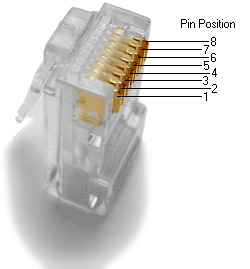
\includegraphics[scale=.7]{png/Rj45plug-8p8c.png}
	\caption{wire numbering on rj45 connector}
	\label{fig:rj45}
\end{figure}

\section{Layer two (nameme osi 2+3)}

\subsection{Busmaster Discovery and Negotiation}
At cold start or when the current busmaster drops out (disconnected, failure), there will be no communication flow on the bus.
When this is detected, the busmaster role must be negotiated between all busmaster capable device.

TODO: Describe busmaster discovery and negotiation.


FIXME: Should there be an announcement of the protocol version in use?
This way an upgrade to more advanced future protocols (e.g. real time capable with timeslots) will be easier.


\subsection{Bus Checking Phase}
During the bus checking phase the busmaster checks which of all registered devices are still alive. For this the busmaster iterates over its internal table of registered devices and sends a paket of type ASKSTAT~\ref{cp:ASKSTAT} to them.

\subsection{Paket Types}
All Pakets of this layer are at least 4 Bytes long and prefixed with the packet delimiter Byte 0x00. 
Since 0x00 is the paket delimiter any 0 Byte in all other fields of a packet  must be escaped

\subsubsection{ASKSTAT}
Busmaster ask a slave for status
\label{cp:ASKSTAT}
\begin{figure}[h!]
\begin{bytefield}{32}
\bitheader{0,7,8,15,16,23,24,31} \\
\small
\bitbox{8}{Type:ASKSTAT}&\bitbox{8}{check8}&\bitbox{16}{Addr:Reciver}
\end{bytefield}
\end{figure}

\subsubsection{STALIVE}
Normal status answer. Slave sends this, if alive, but nothing to say.
\label{cp:STALIVE}
\begin{figure}[h!]
\begin{bytefield}{32}
\bitheader{0,7,8,15,16,23,24,31} \\
\small
\bitbox{8}{Type:STALIVE}&\bitbox{8}{check8}&\bitbox{16}{Addr:Reciver}
\end{bytefield}
\end{figure}


\subsubsection{STALIVPL}
This is similar to STALIVE, but with additional Payload.
\label{cp:STALIVPL}
\begin{figure}[h!]
\begin{bytefield}{32}
\bitheader{0,7,8,15,16,23,24,31} \\
\small
\bitbox{8}{Type:STALIVPL}&\bitbox{8}{check8}&\bitbox{16}{Addr:Reciver}\\
\wordbox{3}{Payload}\\
\end{bytefield}
%Where the Payload is up to 28 bytes of the form:
%\begin{bytefield}{32}
%\bitbox{8}{len}&\bitbox{24}{data\ldots} \\
 %\bitbox{16 CRC16}\\
%\end{bytefield}
\end{figure}


\subsubsection{ASKSTATXXX}
\label{cp:ASKSTATXXX}
\begin{figure}[h!]
\begin{bytefield}{32}
\bitheader{0,7,8,15,16,23,24,31} \\
\small
\bitbox{8}{Type:ASKSTAT}&\bitbox{8}{check8}&\bitbox{16}{Addr:Reciver}
\end{bytefield}
\end{figure}



\section{More Layers}
TODO: specify me!

\newpage
\bibliographystyle{gerplainurl}
%\nocite{LINUX}
\bibliography{spec} 

\end{document}

